\documentclass[tikz]{standalone}
\usepackage{fourier}
\usetikzlibrary{arrows.meta}
\usetikzlibrary{calc}
\tikzset{>=latex}
\definecolor{bookblue}{RGB}{0,173,239}
\definecolor{bookpink}{RGB}{236,0,140}
\definecolor{bookgreen}{RGB}{50,200,0}
\definecolor{bookbluearea}{RGB}{204,239,252}
\tikzstyle{blueline}=[draw=bookblue,line width=0.2mm]
\tikzstyle{pinkline}=[draw=bookpink,line width=0.2mm]
\tikzstyle{greenline}=[draw=bookgreen,line width=0.2mm]
\tikzstyle{blackline}=[draw=black,line width=0.2mm]
\tikzstyle{bluearea}=[fill=bookbluearea]

\begin{document}
  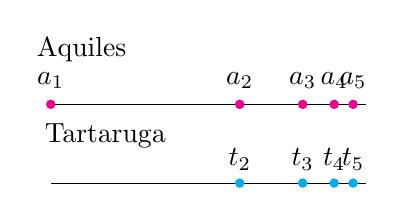
\begin{tikzpicture}
  	\xdef\qtd{4};
  	\xdef\st{1.2};
  	\draw (0,  0) -- (\qtd,  0);
  	\draw (0,-1) -- (\qtd,-1);
  	\node [text width=2cm, anchor=west] at (-0.3,.7) {Aquiles};
  	\node [text width=2cm, anchor=west] at (-0.2,-0.4) {Tartaruga};
  	\foreach \x in {1,...,5}{
  		\fill[bookpink] ({\st*(\qtd - \qtd/\x)},0) circle (0.6mm);
  		\node at ({\st*(\qtd-\qtd/\x)},0.3) {$a_\x$};
  	}
	  \foreach \x in {2,...,5}{
	  	\fill[bookblue] ({\st*(\qtd -\qtd/\x)},-1) circle (0.6mm);
	  	\node at ({\st*(\qtd-\qtd/\x)},-0.7) {$t_\x$};
	  }
  \end{tikzpicture}
\end{document}